\subsection{Radiating Sources in TEM Cells}\label{sec:rad_source_tem}

\subsubsection{Arbitrary source}

Suppose a current $\mathbf{J}_1$ excites the TEM cell, as shown in \autoref{fig:reciprocitytemcell}. Normally, such a current would require external fields to drive it, however, these are neglected here. Only the fields $\mathbf{E}$ and $\mathbf{H}$ radiated by $\mathbf{J}_1$ are considered. These fields satisfy Maxwell's equations \cite[p. 360]{Collin_2015}: 

\begin{subequations}
	\begin{equation}
		\nabla \times \mathbf{E}=-j\omega\mu_0\mathbf{H},
	\end{equation}
	\begin{equation}
		\nabla\times\mathbf{H}=j\omega\epsilon_0\mathbf{E}+\mathbf{J}_1.
	\end{equation}
\end{subequations}


\begin{figure}[htbp]
	\centering
	\includegraphics[width=0.7\linewidth]{content/img/reciprocity_tem_cell}
	\caption{TEM cell with an arbitrary current source $\mathbf{J}_1$ along the line $\boldsymbol{\tau}$. $\mathbf{E}$ and $\mathbf{H}$ are the field intensities induced by the current. $\mathbf{e}^+_n$ and $\mathbf{e}^-_n$ are outgoing fields towards both output ports of the TEM cell. $\mathbf{S}$ indicates the surface, and $V$ the volume of the domain in question.}
	\label{fig:reciprocitytemcell}
\end{figure}

Applying the integral form of the Lorentz reciprocity theorem in \eqref{eqn:lorentz_rec_theorem_int} with $\mathbf{J}_2=\mathbf{M}_1=\mathbf{M}_2=0$ yields

\begin{equation}
	\oiint _S (\mathbf{e}_n^\pm\times \mathbf{H}-\mathbf{E}\times \mathbf{h}_n^\pm)\,d\mathbf{s'}=\iiint \mathbf{J}_1\cdot\mathbf{e}_n^\pm\,dv'.
	\label{eqn:J1_propagating_waves}
\end{equation}

Using the modal expansions \eqref{eqn:a_modal_superposition1} to \eqref{eqn:b_modal_superposition2} for the fields $\mathbf{E}$ and $\mathbf{H}$ radiated by $\mathbf{J}_1$ leads to

\begin{align}
	\oiint _S (\mathbf{e}_n^+\times \mathbf{H}-&\mathbf{E}\times \mathbf{h}_n^+)\,d\mathbf{s'}=\nonumber\\ \nonumber
	&=\oiint _S (\mathbf{e}_n^+\times \sum_m a_m\mathbf{h}_m^+-\sum_m a_m\mathbf{e}_m^+\times \mathbf{h}_n^+)\,d\mathbf{s'}\\
	&=\sum_m a_m \oiint _S (\mathbf{e}_n^+\times \mathbf{h}_m^+-\mathbf{e}_m^+\times \mathbf{h}_n^+)\,d\mathbf{s'}.
\end{align}

Due to the orthogonality condition in \eqref{eqn:norm_power} and the normalization in \eqref{eqn:unit_power}, the coefficients of each mode can be evaluated separately with

\begin{align}
	\oiint _S (\mathbf{e}_n^+\times \mathbf{H}&-\mathbf{E}\times \mathbf{h}_n^+)\,d\mathbf{s'}=\nonumber\\
	&=a_n \oiint _S (\mathbf{e}_n^+\times \mathbf{h}_n^+-\mathbf{e}_n^+\times \mathbf{h}_n^+)\,d\mathbf{s'}=-2a_n.
\end{align}

The coefficient $b_n$ of the fields $\mathbf{e}_n^-$ and $\mathbf{h}_n^-$ is evaluated in the same manner:

\begin{equation}
	b_n=-\frac{1}{2}\iiint \mathbf{J}_1\cdot\mathbf{e}_n^-\,dv'
\end{equation}

Assuming only the TEM mode can propagate, combining \eqref{eqn:unit_power} with the fields $\mathbf{e}_\mathrm{TEM}$ and $\mathbf{h}_\mathrm{TEM}$ with their respective coefficients $a_\mathrm{TEM}$, $b_\mathrm{TEM}$ leads to \cite{4091811}

\begin{subequations}
	\begin{equation}
		P_{\mathrm{out1}}=\iint_S \langle \mathbf{S} \rangle \,d\mathbf{s'}= \iint_S \frac{1}{2} \, \Re \{ \left(a\cdot \mathbf{e}_\mathrm{TEM}^\pm\right) \times \left(a\cdot \mathbf{h}_\mathrm{TEM}^\pm\right)^* \}\,d\mathbf{s'} = \frac{|a_\mathrm{TEM}|^2}{2},
		\label{eqn:power_of_poynting1}
	\end{equation}
	\begin{equation}
		P_{\mathrm{out2}}=\iint_S \langle \mathbf{S} \rangle \,d\mathbf{s'}= \iint_S \frac{1}{2} \, \Re \{ \left(b\cdot \mathbf{e}_\mathrm{TEM}^\pm\right) \times \left(b\cdot \mathbf{h}_\mathrm{TEM}^\pm\right)^* \} \,d\mathbf{s'} = \frac{|b_\mathrm{TEM}|^2}{2}.
		\label{eqn:power_of_poynting2}
	\end{equation}
\end{subequations}

The Poynting vector $\langle \mathbf{S} \rangle$ of the TEM mode in \crefrange{eqn:power_of_poynting1}{eqn:power_of_poynting2} does not have an imaginary component,

\begin{equation}
	\langle \mathbf{S} \rangle=\mathbf{e}_\mathrm{TEM}^\pm\times\mathbf{h}_\mathrm{TEM}^\pm=\Re\{\mathbf{e}_\mathrm{TEM}^\pm\times\left(\mathbf{h}_\mathrm{TEM}^\pm\right)^*\}.
	\label{eqn:equivalent_tem}
\end{equation}

\crefrange{eqn:power_of_poynting1}{eqn:power_of_poynting2} demonstrate that the coefficients $a_\mathrm{TEM}$ and $b_\mathrm{TEM}$ are directly related to the output power. Consequently, the output power can be directly linked to the electric and magnetic field distribution of the TEM mode, and vice versa.

\subsubsection{Equivalent dipole moments}\label{sec:equ-dip-mom}

\cref{eqn:m_e_def,eqn:J1_propagating_waves} relate the electric dipole moment $\mathbf{m}_e$ with a given source current $\mathbf{J}_1$ flowing through an infinitesimal wire, yielding \cite{Sreenivasiah_Chang_Ma_1981}

\begin{equation}
	\begin{pmatrix}a_n \\b_n\end{pmatrix} = -\frac{1}{2}\mathbf{m}_e\cdot \mathbf{e}_n^\pm.
	\label{eqn:dipole_tem_waves}
\end{equation}

If this arbitrary current distribution forms an infinitesimal loop, the source can be represented by a magnetic dipole moment $\mathbf{m}_m$. This leads to \cite{Collin_2015}

\begin{align}
	\begin{pmatrix}a_n \\b_n\end{pmatrix} &= -\oint_C \mathbf{e}_n^\pm \,d\mathbf{l} \nonumber \\
	&= -\iint_{S} \nabla \times \mathbf{e}_n^\pm \,d\mathbf{s'}\nonumber\\
	&= j\omega\mu_0\iint_{S} \mathbf{h}_n^\pm \,d\mathbf{s'}\nonumber\\
	&= j\omega\mu_0\mathbf{m}_m\cdot\mathbf{h}_n^\pm 
	\label{eqn:mag_dipole_moment_tem}
\end{align}

This formulation assumes that the magnetic field strength $\mathbf{h}^\pm$ does not change over the loop area. This is the case for electrically small loops. Otherwise, the magnetic field strength $\mathbf{h}^\pm$ must be considered in the integration process of \eqref{eqn:mag_dipole_moment_tem} \cite{Collin_2015}.

If several modes are propagating, it is useful to determine the coefficients $a_n$ and $b_n$ weighting the modes in \eqref{eqn:a_modal_superposition1} and \eqref{eqn:b_modal_superposition2}. In this case, the orthogonality property in \eqref{eqn:norm_power} can be used to derive \cite{Collin_2015}

\begin{subequations}
	\begin{equation}
		2a_n = -\int_C \boldsymbol{\tau}\cdot\mathbf{e}_n^-\,dl,
		\label{eqn:an}
	\end{equation}
	\begin{equation}
		2b_n = \int_C \boldsymbol{\tau}\cdot\mathbf{e}_n^+\,dl.
		\label{eqn:bn}
	\end{equation}
\end{subequations} 

The wire follows the curve $C$, and $\boldsymbol{\tau}$ is the tangential vector along that curve.

%An electrically small radiating source may be represented by six dipoles. This number includes three magnetic dipoles pointing in every direction of the Cartesian coordinate system (x, y, and z-direction), and three electric dipoles in the same orientation. Consequently, an equipment under test (EUT) could be modeled with these dipoles, leading to much less computational effort in simulation. The excited EM waves by point sources is discussed in \cite{Collin_2015} and in \autoref{sec:modes_tem_cell}. An analytical procedure to determine these dipole moments is presented by Sreenivasiah \cite{Sreenivasiah_Chang_Ma_1981}, and some experimental results based on it can be found in the research of Kreindl, where bond wires were modeled with magnetic dipoles\cite{Kreindl_Bauernfeind_Weiss_Stockreiter_Kaltenbacher_2024}, and, again, Sreenivasiah \cite{Sreenivasiah_Chang_Ma_1981}.

In the presence of both a magnetic and an electric dipole moment, their contributions can be summed, resulting in \cite{Sreenivasiah_Chang_Ma_1981}

\begin{equation}
    \begin{pmatrix}a_n \\b_n\end{pmatrix} = \frac{1}{2}(-\mathbf{m}_e\cdot \mathbf{e}_n^\pm+j\omega\mu_0\mathbf{m}_m\cdot\mathbf{h}_n^\pm).
    \label{eqn:a_b_moments}
\end{equation}

For the TEM mode, the relation between $\mathbf{e}^\pm_\mathrm{TEM}$ and $\mathbf{h}^\pm_\mathrm{TEM}$ expressed in \eqref{eqn:tem_h_e_relation} yields a simplified form of \eqref{eqn:a_b_moments}, written as \cite{Sreenivasiah_Chang_Ma_1981}

\begin{equation}
    \begin{pmatrix}a_\mathrm{TEM} \\b_\mathrm{TEM}\end{pmatrix} =-\frac{1}{2}(\mathbf{m}_e\pm jk\mathbf{m}_m\times \mathbf{z})\cdot \mathbf{e}_\mathrm{TEM}^\pm.
    \label{eqn:a_b_moments_simp}
\end{equation}

Equation \eqref{eqn:a_b_moments_simp} proves useful in later investigations, as it requires knowledge of only $\mathbf{e}^\pm_\mathrm{TEM}$ to determine the dipole moments. The complex magnitude of the dipole moments ${m}_{\mathrm{e}}$ and ${m}_{\mathrm{m}}$ is separately derived by 

\begin{subequations}
\begin{equation}
	{m}_{\mathrm{e}}=\frac{a_\mathrm{TEM}+b_\mathrm{TEM}}{{e}_\mathrm{TEM}^\pm},
	\label{eqn:ifa_me}
\end{equation}

\begin{equation}
	{m}_{\mathrm{m}}=j\frac{a_\mathrm{TEM}-b_\mathrm{TEM}}{k_0 \, {e}_\mathrm{TEM}^\pm}.	
	\label{eqn:ifa_mm}
\end{equation}
\end{subequations}

The individual components of the electric field for a given mode $\mathbf{e}^\pm_n=e_{n,x}^\pm\cdot \mathbf{\hat{a}}_x+e_{n,y}^\pm\cdot \mathbf{\hat{a}}_y+e_{n,z}^\pm\cdot \mathbf{\hat{a}}_z$ can be analyzed separately by examining the output power of the TEM cell. For example, the components of $\mathbf{m}_\mathrm{e}$ are derived with

\begin{subequations}
	\begin{equation}
		 m_{\mathrm{ex}} = \frac{2 \sqrt{P_\mathrm{x}}}{e^\pm_{\mathrm{n,x}}},
		\label{eqn:e0x_mse}
	\end{equation}
	\begin{equation}
		m_{\mathrm{\mathrm{ey}}} = \frac{2 \sqrt{P_\mathrm{y}}}{e^\pm_{\mathrm{n,y}}}.
		\label{eqn:e0y_mse}
	\end{equation}
\end{subequations}

$P_\mathrm{x}$ and $P_\mathrm{y}$ describe the power measured at one output port induced by the respective component of the dipole moment \cite{Sreenivasiah_Chang_Ma_1981}. 

For the TEM mode, an electric dipole placed in the TEM cell leads to output power with the same phase at both ports. This directly results from the symmetric field distribution of the TEM mode leading to the same $\mathbf{e}^\pm_\mathrm{TEM}$ component at the output ports. In contrast, a magnetic dipole results in a phase shift of $\pm\pi$. This difference arises from the phase shift of the magnetic fields at the output ports, $\mathbf{h}_\mathrm{TEM}^+$ and $\mathbf{h}_\mathrm{TEM}^-$, as illustrated in \autoref{fig:reciprocitytemcelltemmode}. 

\begin{figure}[htbp]
	\centering
	\includegraphics[width=0.7\linewidth]{content/img/reciprocity_tem_cell_tem_mode}
	\caption{Field distribution of the TEM mode highlighting the out-of-phase magnetic fields at the output ports.}
	\label{fig:reciprocitytemcelltemmode}
\end{figure}

For the next higher-order mode TE\textsubscript{01}, the situation is reversed. An electric dipole moment leads to a phase shift of $\pm\pi$, while a magnetic dipole moment produces no phase shift. This behavior is due to the asymmetric field distribution of the TE\textsubscript{01} mode, thus a phase shift occurs now between the magnetic field intensities at the output ports, $\mathbf{h}_\mathrm{TE01}^+$ and $\mathbf{h}_\mathrm{TE01}^-$, while there is again no phase shift between the electric field intensities, $\mathbf{e}_\mathrm{TE01}^+$ and $\mathbf{e}_\mathrm{TE01}^-$.

It is assumed that the dipole moments are positioned halfway along the septum in $z$-direction. A shift in $z$-direction introduces a phase shift between the output port powers, consequently altering the results derived above.

%It is required to measure the power at the output ports with phase information, which is done with the complex Poynting vector in a numerical analysis. When measuring an EUT with a real TEM cell, the phase information may be found by summing and subtracting the output powers of the ports, as is shown in \cite{Sreenivasiah_Chang_Ma_1981}.



\subsubsection{Electrically small antennas}\label{sec:el_small_antennas}

The electric field coupling with an electrically small antenna can be expressed as \cite[p. 361]{Collin_2015}

\begin{subequations}
	
	\begin{equation}
		2a_n=-\int_C \boldsymbol{\tau} I(l)\cdot \mathbf{e}_n^+\,dl.
		\label{eqn:e_int_a}
	\end{equation}
	\begin{equation}
		2b_n=-\int_C \boldsymbol{\tau} I(l)\cdot \mathbf{e}_n^-\,dl.
		\label{eqn:e_int_b}
	\end{equation}
	
\end{subequations}

Since the antenna is electrically small, the electric field $\mathbf{e}_n^\pm$ is assumed to be constant in $C$. Furthermore, if the current $I$ is constant along $C$, it does not have to be considered in the integration. Integrating over the closed loop simplifies to \cite[p. 361]{Collin_2015}

\begin{subequations}
	\begin{equation}
		2a_n=-\oint_C \mathbf{e}_n^+\cdot \boldsymbol{\tau}\,dl = j\omega\mu_0 \iint_S \mathbf{h}_n^+\,d\mathbf{s}'=V_n^+,
		\label{eqn:e_a_closed_int}
	\end{equation}
	\begin{equation}
		2b_n=-\oint_C \mathbf{e}_n^-\cdot \boldsymbol{\tau}\,dl = j\omega\mu_0 \iint_S \mathbf{h}_n^-\,d\mathbf{s}'=V_n^-.
		\label{eqn:e_b_closed_int}
	\end{equation}
\end{subequations}

The induced voltage $V_n^+$ is related to the fields $\mathbf{e}_n^+$ and $\mathbf{h}_n^+$ at the output port located in positive $z$-direction, while the induced voltage $V_n^-$ is related to the fields at the other output port $\mathbf{e}_n^-$ and $\mathbf{h}_n^-$. For the TEM mode, the total induced voltage equals $V_\mathrm{TEM}=V_\mathrm{TEM}^--V_\mathrm{TEM}^+$. The relation to the magnitude of the magnetic dipole moment ${m}_m$ is expressed as

\begin{equation}
	m_m=\frac{a_\mathrm{TEM}-b_\mathrm{TEM}}{e_\mathrm{TEM}^\pm\cdot k_0}=\frac{V_\mathrm{TEM}}{{e}_\mathrm{TEM}^\pm\cdot k_0}.
	\label{eqn:m_v}
\end{equation}

For the TE\textsubscript{01} mode, the total induced voltage equals $V_\mathrm{TE01}=V_\mathrm{TE01}^-+V_\mathrm{TE01}^+$. 

In the general case, a magnetic dipole moment $\mathbf{m}_m$ producing fields characterized with coefficients $a_n$ and $b_n$ models the magnetic coupling behavior of any electrically small antenna yielding the same coefficients. Consequently, deriving an equivalent magnetic dipole moment $\mathbf{m}_m$ of an electrically small antenna is possible by measuring $a_n$ and $b_n$ at the output ports. 

In a similar manner to \eqref{eqn:e_int_a} and \eqref{eqn:e_int_b}, a constant magnetic field $\mathbf{h}_n^\pm$ along a magnetic current $I_m$ following a curve $C$ makes the following expression possible:

\begin{subequations}
	
	\begin{equation}
		2a_n=-\int_C \boldsymbol{\tau} I_m(l)\cdot \mathbf{h}_n^+\,dl,
		\label{eqn:h_int_a}
	\end{equation}
	\begin{equation}
		2b_n=-\int_C \boldsymbol{\tau} I_m(l)\cdot \mathbf{h}_n^-\,dl.
		\label{eqn:h_int_b}
	\end{equation}
	
\end{subequations}

Analogous to \eqref{eqn:e_a_closed_int} and \eqref{eqn:e_b_closed_int}, $I_m$ is assumed to be constant and $C$ to form a closed loop, leading to 

\begin{subequations}
	\begin{equation}
		2a_n=-\oint_C \mathbf{h}_n^- \cdot \boldsymbol{\tau}\,dl = -j\omega\epsilon_0 \iint_{S_0} \mathbf{e}_n^+\,d\mathbf{s}',
		\label{eqn:h_a_closed_int}
	\end{equation}
	\begin{equation}
		2b_n=-\oint_C \mathbf{h}_n^+ \cdot \boldsymbol{\tau}\,dl = -j\omega\epsilon_0 \iint_{S_0} \mathbf{e}_n^-\,d\mathbf{s}'.
		\label{eqn:h_b_closed_int}
	\end{equation}
\end{subequations}

Now, the surfaces $S_1$ and $S_2$ are defined, which are depicted in \autoref{fig:displacement-current-tem-cell}. Surface $S_1$ starts from $S_0$ and runs parallel to the electric field $\mathbf{e}_n^\pm$, extending infinitely. A total surface is defined as $S=S_0+S_1+S_2$, where $S_2$ closes the total surface around $S_1$ at infinity. 

\begin{figure}[htbp]
	\centering
	\includegraphics[width=0.75\linewidth]{content/img/displacement-current-tem-cell}
	\caption{Sketch of the surfaces $S_0, S_1$ and $S_2$ in the TEM cell with an example antenna, coupling through $S_0$ to the septum over the displacement current $\partial \mathbf{D}/\partial t$.}
	\label{fig:displacement-current-tem-cell}
\end{figure}

Consequently, \eqref{eqn:h_a_closed_int} and \eqref{eqn:h_b_closed_int} can be written with the newly defined closed surface $S$ as 


\begin{equation}
	j \omega \epsilon_0 \oiint_{S} \mathbf{e}_n^{\pm} \cdot d\mathbf{s'}=j \omega \epsilon_0 \iint_{S_0} \mathbf{e}_n^{\pm} \cdot d\mathbf{s'}+\underbrace{j \omega \epsilon_0 \iint_{S_1} \mathbf{e}_n^{\pm} \cdot d\mathbf{s'}}_{=0}+\underbrace{j \omega \epsilon_0 \iint_{S_2} \mathbf{e}_n^{\pm} \cdot d\mathbf{S}}_{=0}.
\end{equation}

Inserting Gauss' law $\nabla\cdot \mathbf{E}=\frac{\rho}{\epsilon_0}$ leads to

\begin{equation}
	-j \omega \epsilon_0 \oiint_{S} \mathbf{e}_n^{\pm} \cdot d\mathbf{s'} = -j \omega \epsilon_0 \iiint_{V} \nabla \cdot\mathbf{e}_n^{\pm} \cdot dv' = -j \omega \iiint_{V} {\rho}_n^\pm \cdot dv'.
\end{equation}

With the continuity equation $j\omega\rho = -\nabla\cdot \mathbf{J}$ this yields

\begin{subequations}
	\begin{equation}
		2a_n = -j \omega \iiint_{V} {\rho}_n^+ \cdot dv' = \iiint_{V} \nabla \cdot \mathbf{J}_n^+ \cdot dv' = \oiint_{S} \mathbf{J}_n^+ \cdot d\mathbf{s'} =I_n^+,
		\label{eqn:charges_a}
	\end{equation}
	\begin{equation}
		2b_n = -j \omega \iiint_{V} {\rho}_n^- \cdot dv' = \iiint_{V} \nabla \cdot \mathbf{J}_n^- \cdot dv' = \oiint_{S} \mathbf{J}_n^- \cdot d\mathbf{s'} = I_n^-.
		\label{eqn:charges_b}
	\end{equation}
\end{subequations}

For the TEM mode, the electric dipole moment magnitude ${m}_e$ can be expressed in terms of the total current $I_\mathrm{TEM}=I_\mathrm{TEM}^+ + I_\mathrm{TEM}^-$ by substituting \eqref{eqn:charges_a} and \eqref{eqn:charges_b} into \eqref{eqn:ifa_me}, yielding
\begin{equation}
	{m}_e=\frac{a_\mathrm{TEM}+b_\mathrm{TEM}}{{e}_\mathrm{TEM}^\pm}=\frac{I_\mathrm{TEM}}{{e}_\mathrm{TEM}^\pm}.
	\label{eqn:me_i}
\end{equation}

An electric dipole moment $\mathbf{m}_e$ producing fields characterized with coefficients $a_n$ and $b_n$ models the electric coupling behavior of any electrically small antenna yielding the same coefficients. Consequently, deriving an equivalent $\mathbf{m}_e$ of an electrically small antenna is possible by measuring $a_n$ and $b_n$ at the output port, analogous to the case of $\mathbf{m}_m$. 

The physical meaning of $I_n$ is the electrical current passing between the septum and the dipole via capacitive coupling, representing the displacement current. In summary, the magnetic dipole moment arises from the induced voltage on the septum, whereas the electric dipole moment results from the coupling displacement current.

%%Numerical simulations enable the determination of the combined coefficients $a+b$ and $a-b$ directly. When applying this described method in a measurement with a real TEM cell, the values are found by adding and subtracting the output powers of both ports. The detailed procedure can be found in \cite{Sreenivasiah_Chang_Ma_1981}.
%
%\subsubsection{Radiation resistance}
%
%\todo[inline]{TODO: Dieses Kapitel eventuell rausnehmen.}
%
%The radiation resistance of an electrically small antenna is derived by applying the Green's function. The following content is mostly taken from \cite{4091747}.
%
%To analyze the fields in a TEM cell, the dyadic Green's function discussed in \autoref{sec:dyad_green} proofs itself to be useful. It is assumed, that a vertical, electrically short antenna is inserted in the top center of the TEM cell. This is modeled by a current distribution in y-direction $\mathbf{\hat J}(\mathbf{x}) = \mathbf{a}_y J(\mathbf{x})$ \cite{4091747}. Accordingly, the Green's function reduces to $\mathbf{\hat G}(\mathbf{x, x'}) = \mathbf{a}_y G(\mathbf{x, x'})$. \todo{Check Vector notation. Is correct for Dyadics?} First, the Green's function for a rectangular waveguide $G_O(\mathbf{x,x'})$ is shown in \autoref{eqn:unperturbed_green} \cite{Balanis_1997}. There, $\eta_0$ is the free-space impedance, $M=m\pi / (2a)$, $N=n\pi/b$ and $K_m=(\xi^2-M^2)^{1/2}$. Furthermore,
%
%$\Delta_n = 
%\begin{cases}
%	\frac{1}{2}, & n = 0 \\
%	1,           & n > 0
%\end{cases} $ 
%
%and,
%
%$g_{mn}(\mathbf{x}_t, \mathbf{x}_t') = \left( \frac{2}{ab} \right)
%\sin M(x + a) \sin M(x' + a)
%\cdot \cos Ny \cos Ny'$
%
%are functions implemented in 
%
%\begin{equation}
%	\tilde{G}_0(\mathbf{x}_t, \mathbf{x}_t') =
%	\frac{-\mathrm{j} \eta_0}{k_0} \left\{\sum_{m,n=0}^{\infty} \frac{\Delta_n [M^2 + \beta^2]}{M^2 + N^2 - \xi^2} \; g_{mn}(\mathbf{x}_t, \mathbf{x}_t').
%	\right\}
%	\label{eqn:unperturbed_green}
%\end{equation}
%
%The components $x$, $x'$ and $y$, $y'$ are part of the vectors $\mathbf{x}_t$, $\mathbf{x}'_t$. 
%
%
%\begin{figure}[h]
%	\centering
%	\includegraphics[width=0.7\linewidth]{content/img/vertical_antenna_tem_cell}
%	\caption{TEM cell with vertical antenna inserted}
%	\label{fig:verticalantennatemcell}
%\end{figure}
%
%
%The TEM cells Green's function by adding a unperturbed term to it \cite{4091747}. The derivation of those Green's Functions is demonstrated in \cite{Wilson_1981}, which uses the same methods described in \cite{Balanis_1997}, as mentioned above.
%
%The perturbed term in
%
%\begin{equation}
%	\widetilde{G}_g(\mathbf{x}_t, \mathbf{x}'_t) = \frac{ -j \pi k_0 \eta_0}{2 a^2 s^2} L(\beta) f(\mathbf{x}_t) f(\mathbf{x}'_t)
%	\label{eqn:perturbed_green}
%\end{equation} 
%
%describes the influence of the gaps on the field distribution. They are derived by forcing the tangential fields to be continuous across the gaps, then describing this boundary condition mathematically as a perturbing second Green's function. The rest of the boundary conditions on the are zero due to the geometry of the TEM cell. The functions used are,
%
%\begin{equation*}
%	L(\beta) = \left[
%	\ln \left( \frac{8a}{\pi g} \right)
%	- \frac{\pi}{a} \sum_{m \in \{1,3,5,...\}}^{\infty} \left(
%	\frac{\cot K_m b}{K_m}
%	+ \frac{2a}{m\pi}
%	\right)
%	\right]^{-1}
%\end{equation*}
%
%and, 
%
%\begin{equation*}
%	f(\mathbf{x}_t) = \sum_{m \in \{1,3,5,...\}}^{\infty} M \frac{\cos K_{m} (b - y)}{K_{m} \sin K_{m} b}
%	\sin Ma \cos Mx J_0(Mg).
%\end{equation*}
%
%To receive the final Green's Function, the unperturbed and perturbed term are added together ${G}(\mathbf{x}_t, \mathbf{x}'_t) = {G}_O(\mathbf{x}_t, \mathbf{x}'_t)+{G}_g(\mathbf{x}_t, \mathbf{x}'_t)$. Naturally, the observation point $\mathbf{x}$ can only be on the upper half in the chamber, where the source is also located \cite{4091747}. 
%
%
%
%Because waves propagating in the TEM cell are assumed to travel into infinity, they might have any longitudinal propagation constant $\beta$. They are not limited by boundary conditions in this direction. It therefore proofs useful to apply a Fourier Series over this variable, as done in
%
%\begin{subequations}\label{eqn:greens_fourier}
%	\begin{equation}
%		G_O(\mathbf{x,x'})=\frac{1}{2\pi}\int^\infty_{-\infty} \tilde{G}_0(\mathbf{x_t,x_t'})\mathrm{e}^{j\beta z}\mathrm{d}\beta,
%	\end{equation}
%	\begin{equation}
%		G_g(\mathbf{x,x'})=\frac{1}{2\pi}\int^\infty_{-\infty} \tilde{G}_g(\mathbf{x_t,x_t'})\mathrm{e}^{j\beta z}\mathrm{d}\beta.
%	\end{equation}
%\end{subequations}
%
%Now, the antenna impedance is calculated using 
%
%\begin{equation}\label{eqn:antenna_imp}
%	Z = \frac{-1}{I^2} \int_S \int_{S'} \mathbf{J}(\mathbf{x}) \cdot \mathbf{G}(\mathbf{x}, \mathbf{x}') \cdot \mathbf{J}(\mathbf{x}') \, \mathrm{d}s' \, \mathrm{d}s.
%\end{equation}
%
%The Green's Function in this represents the electric field excited by an unit strength dipole \cite{4091747}. Scaled by multiplication with the current density  $\mathbf{J}(\mathbf{x})$ and integrated over the length of the wire, results in the total electric field. Next, by multiplying it by the current distribution $\mathbf{J}(\mathbf{x})$ and integrated over the length of the wire again, leads to the apparent power. In the end, dividing this term by the total current consumption squared $I^2$ leads to the impedance.
%
%When evaluating the real part of the impedance for the case described here, the radiation resistance results from 
%
%\begin{equation}\label{eqn:rad_res}
%	R = \frac{ \pi \eta_0 k_0^2 }{ 4 a^2 } \csc^2{ k_0 d } \, L(k_0) H(k_0).
%\end{equation}
%
%If the inserted antenna is electrically small, as it is in this case, $d$ reduces the influence of other terms. The most dominant term then, $k_0^2$, results in a quadratic relation of the radiation resistance to the frequency. This agrees with the theoretical framework in the discussion about small dipoles in \cref{sec:dipoles}, as well as with the simulations results in \cref{sec:simulations}.
%
%Here, 
%\begin{equation*}
%	H(\beta) = \sum_{m' \in \{1,3,5,...\}}^{\infty} h_{m'}(\beta) \sum_{m \in \{1,3,5,...\}}^{\infty} h_m(\beta) J_0(r(M^2 + \beta^2)^{1/2})
%\end{equation*}
%
%and,
%
%\begin{equation*}
%	h_m(\beta) = \frac{M \sin Ma J_0(Mg)}{K_m \sin K_m b} \cdot 
%	\frac{\cos k_0 d - \cos K_m d}{M^2 + \beta^2}.
%\end{equation*}



% In reality, at frequencies over cut-off frequencies of TE and TM modes, the dipoles not aligned with the TEM mode will generate some TE/TM modes, which enable them to transmit power and disturb the results, as in \cite{Kreindl_Bauernfeind_Weiss_Stockreiter_Yenumula_Narayanan_Kaltenbacher_2022}.
 
%Furthermore, in the optimal case, the EUT is placed in the dead center of the TEM cell, where the x- and z-component of $\mathbf{e_0}$ in the y=0 plane becomes zero due to symmetry \cite{Sreenivasiah_Chang_Ma_1981}. If this is not the case, the measurements may vary significantly \cite{Kreindl_Bauernfeind_Weiss_Stockreiter_Yenumula_Narayanan_Kaltenbacher_2022}.

%The formula has originally been derived for cylindrical waveguides \cite{Collin_2015}. There, the position of the electric and magnetic dipole moments do not matter, as long as the matching electric and magnetic fields at the surfaces are chosen. This is because the field components do not change direction when propagating from the dipoles to the surfaces, due to the symmetrical property of the cylindrical waveguide. This is not the case for a TEM cell. There, an offset into the x- and y-direction from the center leads to field components, which change direction while traveling to the surfaces. Then, the vector product used in the derivation by Lorentz Reciprocity theorem is not valid anymore. Instead, the fields at the test points have to be considered, and because they don't have a singular x,y or z-component anymore, several more dipole moments become relevant.



%\todo[inline]{This analysis might be wrong. The normalized E-Field is something different here than previously - I mixed it up. What could work: Simulate electric dipole moment in y-direction with geometry sweep. Adjust $y_0$ in \cite{Sreenivasiah_Chang_Ma_1981}. Find norm. E-Field for that. Simulate output power. Compare with calculations.}



\FloatBarrier
